% Options for packages loaded elsewhere
\PassOptionsToPackage{unicode}{hyperref}
\PassOptionsToPackage{hyphens}{url}
%
\documentclass[
]{article}
\usepackage{amsmath,amssymb}
\usepackage{lmodern}
\usepackage{iftex}
\ifPDFTeX
  \usepackage[T1]{fontenc}
  \usepackage[utf8]{inputenc}
  \usepackage{textcomp} % provide euro and other symbols
\else % if luatex or xetex
  \usepackage{unicode-math}
  \defaultfontfeatures{Scale=MatchLowercase}
  \defaultfontfeatures[\rmfamily]{Ligatures=TeX,Scale=1}
\fi
% Use upquote if available, for straight quotes in verbatim environments
\IfFileExists{upquote.sty}{\usepackage{upquote}}{}
\IfFileExists{microtype.sty}{% use microtype if available
  \usepackage[]{microtype}
  \UseMicrotypeSet[protrusion]{basicmath} % disable protrusion for tt fonts
}{}
\makeatletter
\@ifundefined{KOMAClassName}{% if non-KOMA class
  \IfFileExists{parskip.sty}{%
    \usepackage{parskip}
  }{% else
    \setlength{\parindent}{0pt}
    \setlength{\parskip}{6pt plus 2pt minus 1pt}}
}{% if KOMA class
  \KOMAoptions{parskip=half}}
\makeatother
\usepackage{xcolor}
\IfFileExists{xurl.sty}{\usepackage{xurl}}{} % add URL line breaks if available
\IfFileExists{bookmark.sty}{\usepackage{bookmark}}{\usepackage{hyperref}}
\hypersetup{
  pdftitle={Percentage Delay Rate: QuickPay (2009-2012)},
  hidelinks,
  pdfcreator={LaTeX via pandoc}}
\urlstyle{same} % disable monospaced font for URLs
\usepackage[margin=1in]{geometry}
\usepackage{graphicx}
\makeatletter
\def\maxwidth{\ifdim\Gin@nat@width>\linewidth\linewidth\else\Gin@nat@width\fi}
\def\maxheight{\ifdim\Gin@nat@height>\textheight\textheight\else\Gin@nat@height\fi}
\makeatother
% Scale images if necessary, so that they will not overflow the page
% margins by default, and it is still possible to overwrite the defaults
% using explicit options in \includegraphics[width, height, ...]{}
\setkeys{Gin}{width=\maxwidth,height=\maxheight,keepaspectratio}
% Set default figure placement to htbp
\makeatletter
\def\fps@figure{htbp}
\makeatother
\setlength{\emergencystretch}{3em} % prevent overfull lines
\providecommand{\tightlist}{%
  \setlength{\itemsep}{0pt}\setlength{\parskip}{0pt}}
\setcounter{secnumdepth}{5}
\usepackage{booktabs,longtable,dcolumn} \usepackage{multirow,array} \usepackage{wrapfig,float} \floatplacement{figure}{H}
\ifLuaTeX
  \usepackage{selnolig}  % disable illegal ligatures
\fi

\title{Percentage Delay Rate: QuickPay (2009-2012)}
\author{}
\date{\vspace{-2.5em}Mar 10, 2022}

\begin{document}
\maketitle

\hypertarget{percentage-delays-over-time}{%
\section{Percentage delays over
time}\label{percentage-delays-over-time}}

\begin{itemize}
\tightlist
\item
  Sample restricted to projects for which start dates matches the one in
  API

  \begin{itemize}
  \tightlist
  \item
    This is done by using first reported ``action\_date'' and
    ``date\_signed''
  \end{itemize}
\item
  \(PercentDelay_{it}=100 \times Delay_{it}/Duration_{i,t-1}\)

  \begin{itemize}
  \tightlist
  \item
    \(Duration_{i,t-1} = Deadline_{i,t-1} - StartDate_i\)
  \end{itemize}
\end{itemize}

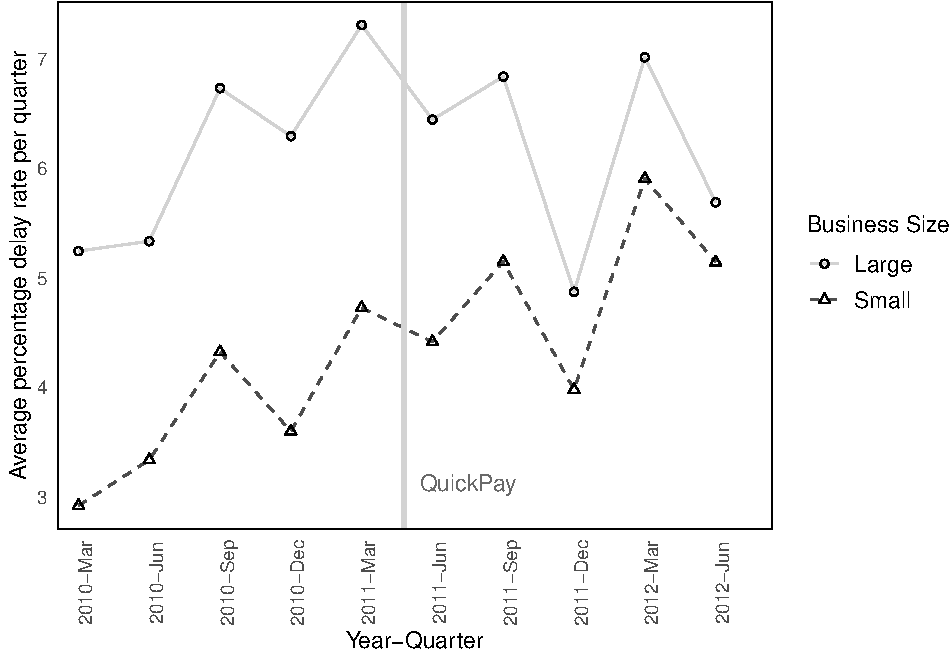
\includegraphics{qp_first_pc_delay-2_files/figure-latex/plot_pc_delay-1.pdf}

\hypertarget{normalized-delay-rate-in-percentage}{%
\subsection{Normalized delay rate (in
percentage)}\label{normalized-delay-rate-in-percentage}}

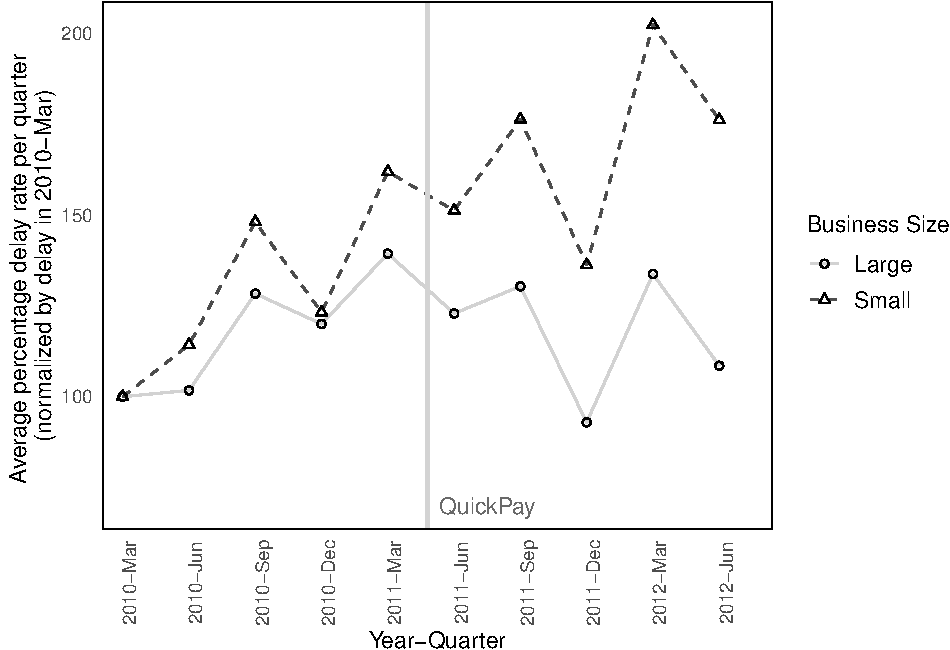
\includegraphics{qp_first_pc_delay-2_files/figure-latex/normalized_plot-1.pdf}

\hypertarget{baseline-regressions}{%
\section{Baseline Regressions}\label{baseline-regressions}}

\[ PercentDelay_{it} = \beta_0 + \beta_1 Treat_i + \beta_2 Post_t + \beta_3 (Treat_i \times Post_t) + e_{it}\]

\[ \begin{aligned} PercentDelay_{it} &=& \alpha+\beta_0 Treat_i + \beta_1 Post_t + \beta_2 (Treat_i \times Post_t)\\
&+&  X_i + (Post_t \times X_i) + \mu_t + \theta_{firm} + \lambda_{task}+ \epsilon_{it}
\end{aligned}\]

\begin{table}[H] \centering 
  \caption{Effect of QuickPay on project delay rates} 
  \label{} 
\small 
\begin{tabular}{@{\extracolsep{-2pt}}lccccc} 
\\[-1.8ex]\hline 
\hline \\[-1.8ex] 
\\[-1.8ex] & \multicolumn{5}{c}{$PercentDelay_{it}$} \\ 
\\[-1.8ex] & (1) & (2) & (3) & (4) & (5)\\ 
\hline \\[-1.8ex] 
 $Treat_i$ & $-$4.76$^{***}$ & $-$3.12$^{***}$ & $-$3.16$^{***}$ & $-$2.43$^{***}$ & $-$2.46$^{***}$ \\ 
  & (0.22) & (0.18) & (0.18) & (0.18) & (0.18) \\ 
  & & & & & \\ 
 $Post_t$ & $-$1.59$^{***}$ & $-$20.02$^{***}$ &  &  &  \\ 
  & (0.21) & (1.51) &  &  &  \\ 
  & & & & & \\ 
 $Treat_i \times Post_t$ & 2.58$^{***}$ & 1.98$^{***}$ & 2.02$^{***}$ & 2.16$^{***}$ & 2.31$^{***}$ \\ 
  & (0.26) & (0.23) & (0.23) & (0.23) & (0.23) \\ 
  & & & & & \\ 
 Constant & 11.03$^{***}$ & 97.03$^{***}$ &  &  &  \\ 
  & (0.18) & (1.14) &  &  &  \\ 
  & & & & & \\ 
\hline \\[-1.8ex] 
Duration, Budget, Bids & No & Yes & Yes & Yes & Yes \\ 
$Post_t \times$  (Duration, Budget, Bids) & No & Yes & Yes & Yes & Yes \\ 
Project stage & No & Yes & Yes & Yes & Yes \\ 
Year-Quarter fixed effects & No & No & Yes & Yes & Yes \\ 
Task fixed effects & No & No & No & Yes & Yes \\ 
Industry fixed effects & No & No & No & No & Yes \\ 
Observations & 260,056 & 235,960 & 235,960 & 235,960 & 235,960 \\ 
R$^{2}$ & 0.003 & 0.24 & 0.24 & 0.28 & 0.28 \\ 
Adjusted R$^{2}$ & 0.003 & 0.24 & 0.24 & 0.27 & 0.28 \\ 
\hline 
\hline \\[-1.8ex] 
\textit{Note:}  & \multicolumn{5}{r}{$^{*}$p$<$0.1; $^{**}$p$<$0.05; $^{***}$p$<$0.01} \\ 
 & \multicolumn{5}{r}{Each observation is a project-quarter.} \\ 
 & \multicolumn{5}{r}{SEs are robust and clustered at the project level.} \\ 
\end{tabular} 
\end{table}

\hypertarget{project-stage}{%
\section{Project Stage}\label{project-stage}}

\begin{itemize}
\tightlist
\item
  \(t\) indicates the end of the quarter
\item
  We want to get stage of the project at the beginning of a given
  quarter (before any delays materialize)
\end{itemize}

\(Stage_{it}=\frac{ActionDate_{t-1}-StartDate_i}{Duration_{i,t-1}}\)
\(Stage_{it}=\frac{(t-1)-StartDate_i}{Duration_{i,t-1}}\)

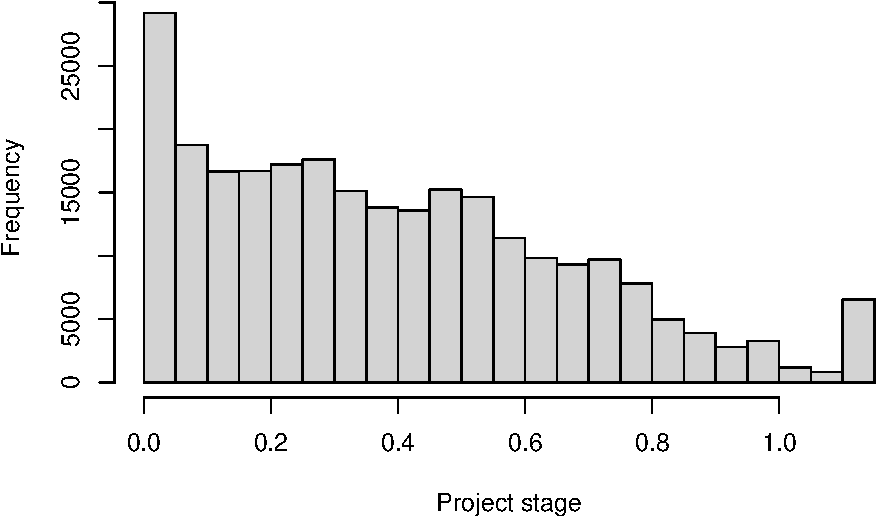
\includegraphics{qp_first_pc_delay-2_files/figure-latex/stage_plots_1-1.pdf}

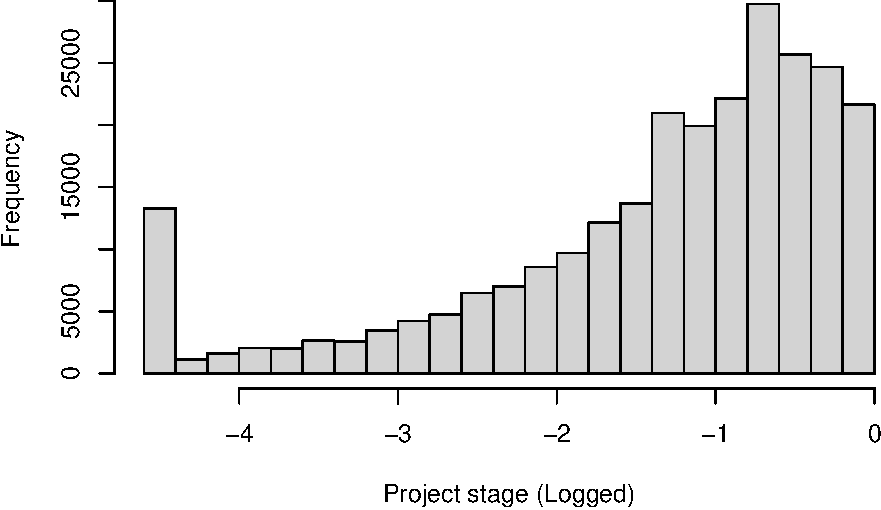
\includegraphics{qp_first_pc_delay-2_files/figure-latex/stage_plots_2-1.pdf}

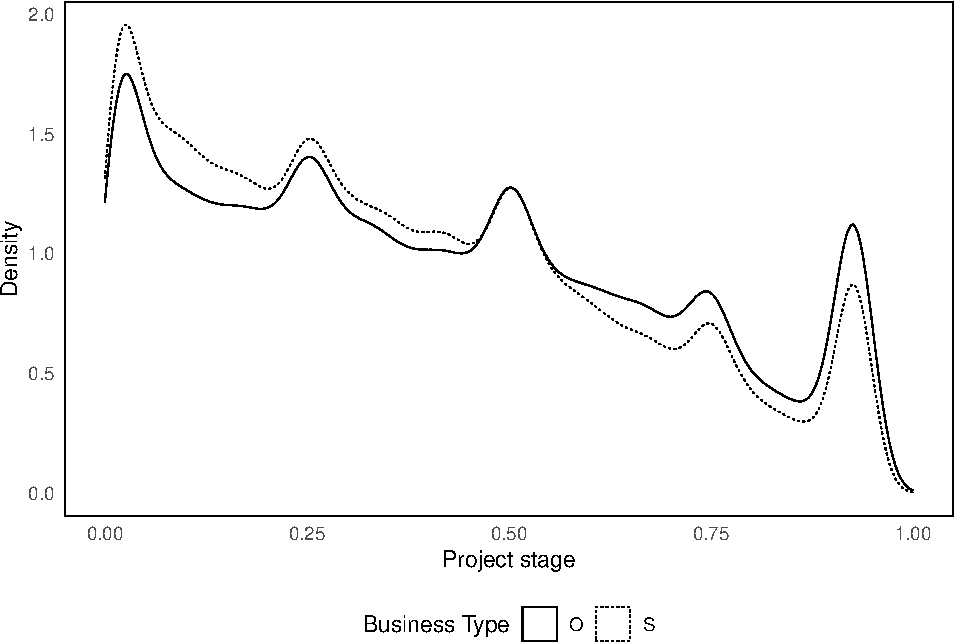
\includegraphics{qp_first_pc_delay-2_files/figure-latex/stage_plots_3-1.pdf}

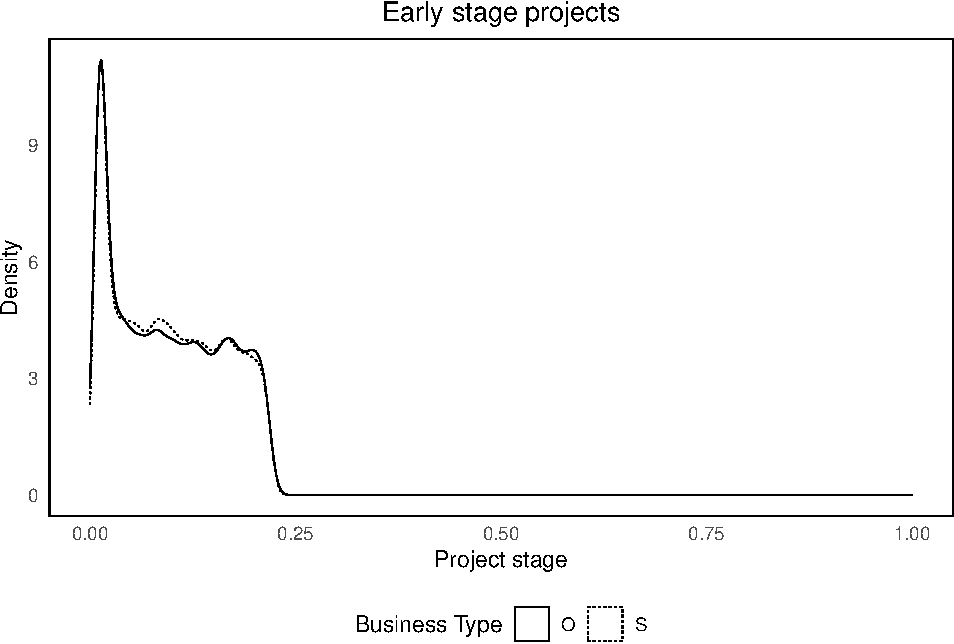
\includegraphics{qp_first_pc_delay-2_files/figure-latex/stage_plots_tercile_1-1.pdf}

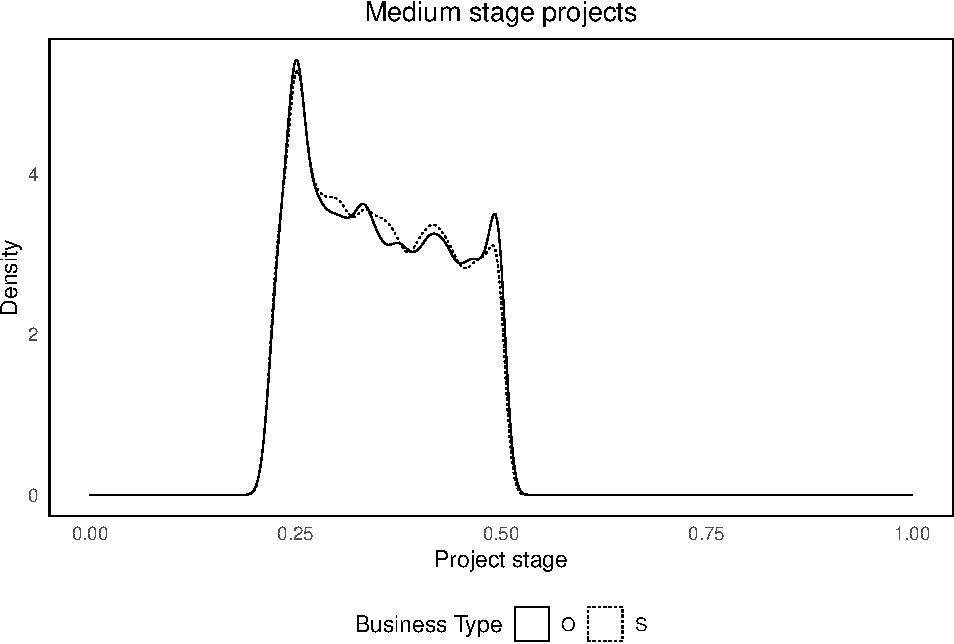
\includegraphics{qp_first_pc_delay-2_files/figure-latex/stage_plots_tercile_2-1.pdf}

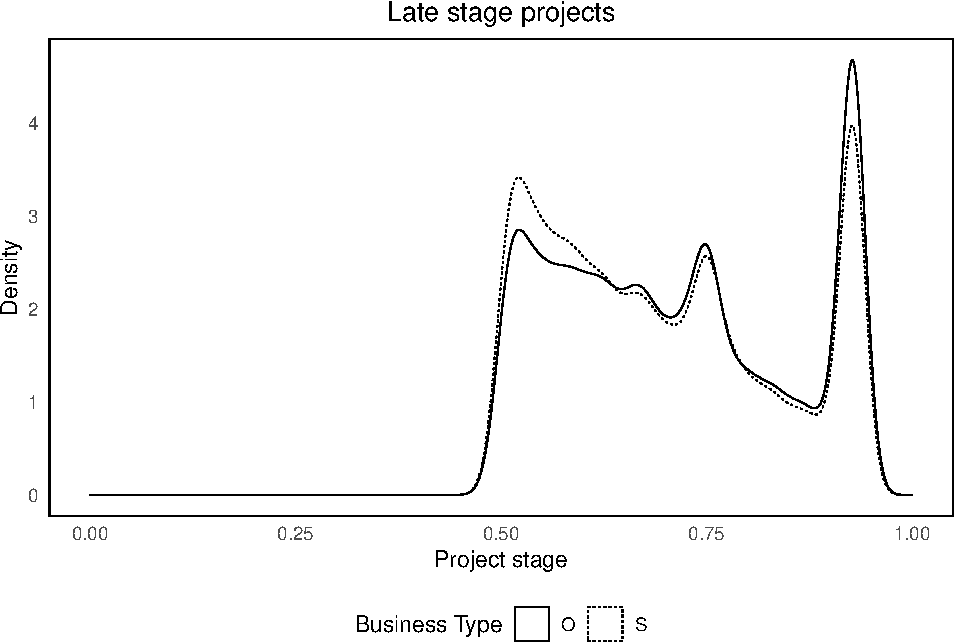
\includegraphics{qp_first_pc_delay-2_files/figure-latex/stage_plots_tercile_3-1.pdf}

\begin{table}[H] \centering 
  \caption{Project Stage and QuickPay reform} 
  \label{} 
\small 
\begin{tabular}{@{\extracolsep{-2pt}}lccccc} 
\\[-1.8ex]\hline 
\hline \\[-1.8ex] 
\\[-1.8ex] & \multicolumn{5}{c}{$PercentDelay_{it}$  } \\ 
\\[-1.8ex] & (1) & (2) & (3) & (4) & (5)\\ 
\hline \\[-1.8ex] 
 $Treat_i$ & $-$0.64$^{***}$ & $-$2.56$^{***}$ & $-$2.51$^{***}$ & $-$1.85$^{***}$ & $-$1.80$^{***}$ \\ 
  & (0.15) & (0.21) & (0.21) & (0.21) & (0.21) \\ 
  & & & & & \\ 
 Medium Stage & 1.35$^{***}$ & 0.20 & $-$0.02 & 0.55$^{**}$ & 0.54$^{**}$ \\ 
  & (0.20) & (0.23) & (0.23) & (0.23) & (0.23) \\ 
  & & & & & \\ 
 Late Stage & 30.39$^{***}$ & 18.95$^{***}$ & 18.72$^{***}$ & 18.23$^{***}$ & 18.25$^{***}$ \\ 
  & (0.54) & (0.41) & (0.42) & (0.41) & (0.41) \\ 
  & & & & & \\ 
 $Post_t$ & $-$0.31$^{**}$ & $-$16.51$^{***}$ &  &  &  \\ 
  & (0.16) & (1.48) &  &  &  \\ 
  & & & & & \\ 
 $Treat_i \times Post_t$ & 0.31 & 0.28 & 0.25 & 0.31 & 0.44$^{*}$ \\ 
  & (0.20) & (0.27) & (0.27) & (0.26) & (0.26) \\ 
  & & & & & \\ 
 $Treat_i \times$ Medium Stage & $-$0.79$^{***}$ & 0.82$^{***}$ & 0.79$^{***}$ & 0.63$^{**}$ & 0.63$^{**}$ \\ 
  & (0.25) & (0.28) & (0.28) & (0.28) & (0.28) \\ 
  & & & & & \\ 
 $Treat_i \times$ Late Stage & $-$10.79$^{***}$ & $-$2.73$^{***}$ & $-$2.84$^{***}$ & $-$3.09$^{***}$ & $-$3.33$^{***}$ \\ 
  & (0.68) & (0.55) & (0.55) & (0.54) & (0.54) \\ 
  & & & & & \\ 
 $Post_t \times$ Medium Stage & $-$1.38$^{***}$ & 0.89$^{***}$ & 0.70$^{**}$ & 0.12 & 0.12 \\ 
  & (0.24) & (0.28) & (0.29) & (0.28) & (0.28) \\ 
  & & & & & \\ 
 $Post_t \times$ Late Stage & $-$12.27$^{***}$ & $-$4.24$^{***}$ & $-$4.36$^{***}$ & $-$5.15$^{***}$ & $-$5.18$^{***}$ \\ 
  & (0.61) & (0.48) & (0.49) & (0.48) & (0.48) \\ 
  & & & & & \\ 
 $Treat_i \times Post_t \times$ Medium Stage & 0.77$^{***}$ & $-$0.16 & $-$0.17 & 0.15 & 0.14 \\ 
  & (0.30) & (0.36) & (0.36) & (0.35) & (0.35) \\ 
  & & & & & \\ 
 $Treat_i \times Post_t \times$ Late Stage & 8.09$^{***}$ & 4.89$^{***}$ & 4.97$^{***}$ & 5.26$^{***}$ & 5.40$^{***}$ \\ 
  & (0.77) & (0.66) & (0.66) & (0.65) & (0.65) \\ 
  & & & & & \\ 
 Constant & 2.28$^{***}$ & 82.74$^{***}$ &  &  &  \\ 
  & (0.12) & (1.13) &  &  &  \\ 
  & & & & & \\ 
\hline \\[-1.8ex] 
Duration, Budget, Bids & No & Yes & Yes & Yes & Yes \\ 
$Post_t \times $  (Duration, Budget, Bids) & No & Yes & Yes & Yes & Yes \\ 
Year-Quarter fixed effects & No & No & Yes & Yes & Yes \\ 
Task fixed effects & No & No & No & Yes & Yes \\ 
Industry fixed effects & No & No & No & No & Yes \\ 
Observations & 260,000 & 235,960 & 235,960 & 235,960 & 235,960 \\ 
R$^{2}$ & 0.10 & 0.27 & 0.27 & 0.29 & 0.30 \\ 
Adjusted R$^{2}$ & 0.10 & 0.27 & 0.27 & 0.29 & 0.29 \\ 
\hline 
\hline \\[-1.8ex] 
\textit{Note:}  & \multicolumn{5}{r}{$^{*}$p$<$0.1; $^{**}$p$<$0.05; $^{***}$p$<$0.01} \\ 
 & \multicolumn{5}{r}{Each observation is a project-quarter.} \\ 
 & \multicolumn{5}{r}{SEs are robust and clustered at the project level.} \\ 
\end{tabular} 
\end{table}

\begin{table}[H] \centering 
  \caption{Project Stage and QuickPay reform} 
  \label{} 
\small 
\begin{tabular}{@{\extracolsep{-2pt}}lccccc} 
\\[-1.8ex]\hline 
\hline \\[-1.8ex] 
\\[-1.8ex] & \multicolumn{5}{c}{$PercentDelay_{it}$  } \\ 
\\[-1.8ex] & (1) & (2) & (3) & (4) & (5)\\ 
\hline \\[-1.8ex] 
 $Treat_i$ & $-$8.65$^{***}$ & $-$4.13$^{***}$ & $-$4.19$^{***}$ & $-$3.34$^{***}$ & $-$3.46$^{***}$ \\ 
  & (0.44) & (0.34) & (0.34) & (0.34) & (0.33) \\ 
  & & & & & \\ 
 Log(Stage) & 6.19$^{***}$ & 3.84$^{***}$ & 3.76$^{***}$ & 3.83$^{***}$ & 3.84$^{***}$ \\ 
  & (0.14) & (0.11) & (0.11) & (0.11) & (0.11) \\ 
  & & & & & \\ 
 $Post_t$ & $-$4.77$^{***}$ & $-$19.54$^{***}$ &  &  &  \\ 
  & (0.42) & (1.53) &  &  &  \\ 
  & & & & & \\ 
 $Treat_i \times Post_t$ & 5.30$^{***}$ & 3.26$^{***}$ & 3.30$^{***}$ & 3.49$^{***}$ & 3.71$^{***}$ \\ 
  & (0.51) & (0.43) & (0.43) & (0.42) & (0.42) \\ 
  & & & & & \\ 
 $Treat_i \times$ Log(Stage) & $-$2.65$^{***}$ & $-$0.59$^{***}$ & $-$0.61$^{***}$ & $-$0.54$^{***}$ & $-$0.60$^{***}$ \\ 
  & (0.17) & (0.15) & (0.15) & (0.14) & (0.14) \\ 
  & & & & & \\ 
 $Post_t \times$ Log(Stage) & $-$0.82$^{***}$ & 0.75$^{***}$ & 0.75$^{***}$ & 0.31$^{**}$ & 0.29$^{**}$ \\ 
  & (0.17) & (0.14) & (0.14) & (0.14) & (0.14) \\ 
  & & & & & \\ 
 $Treat_i \times Post_t \times$ Log(Stage) & 1.46$^{***}$ & 0.77$^{***}$ & 0.79$^{***}$ & 0.86$^{***}$ & 0.90$^{***}$ \\ 
  & (0.21) & (0.19) & (0.19) & (0.18) & (0.18) \\ 
  & & & & & \\ 
 Constant & 21.00$^{***}$ & 97.14$^{***}$ &  &  &  \\ 
  & (0.36) & (1.15) &  &  &  \\ 
  & & & & & \\ 
\hline \\[-1.8ex] 
Duration, Budget, Bids & No & Yes & Yes & Yes & Yes \\ 
$Post_t \times $  (Duration, Budget, Bids) & No & Yes & Yes & Yes & Yes \\ 
Year-Quarter fixed effects & No & No & Yes & Yes & Yes \\ 
Task fixed effects & No & No & No & Yes & Yes \\ 
Industry fixed effects & No & No & No & No & Yes \\ 
Observations & 260,000 & 235,960 & 235,960 & 235,960 & 235,960 \\ 
R$^{2}$ & 0.05 & 0.24 & 0.25 & 0.28 & 0.28 \\ 
Adjusted R$^{2}$ & 0.05 & 0.24 & 0.25 & 0.27 & 0.28 \\ 
\hline 
\hline \\[-1.8ex] 
\textit{Note:}  & \multicolumn{5}{r}{$^{*}$p$<$0.1; $^{**}$p$<$0.05; $^{***}$p$<$0.01} \\ 
 & \multicolumn{5}{r}{Each observation is a project-quarter.} \\ 
 & \multicolumn{5}{r}{SEs are robust and clustered at the project level.} \\ 
\end{tabular} 
\end{table}

\hypertarget{aliter-stage-definition}{%
\subsection{Aliter: Stage definition}\label{aliter-stage-definition}}

\begin{itemize}
\tightlist
\item
  \(t\) indicates the end of the quarter
\end{itemize}

\(Stage_{it}=\frac{ActionDate_{t}-StartDate_i}{Duration_{i,t}}\)
\(Stage_{it}=\frac{t-StartDate_i}{Duration_{i,t}}\)

\begin{table}[H] \centering 
  \caption{Project Stage and QuickPay reform} 
  \label{} 
\small 
\begin{tabular}{@{\extracolsep{-2pt}}lccccc} 
\\[-1.8ex]\hline 
\hline \\[-1.8ex] 
\\[-1.8ex] & \multicolumn{5}{c}{$PercentDelay_{it}$  } \\ 
\\[-1.8ex] & (1) & (2) & (3) & (4) & (5)\\ 
\hline \\[-1.8ex] 
 $Treat_i$ & $-$2.36$^{***}$ & $-$1.34$^{***}$ & $-$1.08$^{**}$ & $-$1.13$^{**}$ & $-$1.15$^{**}$ \\ 
  & (0.35) & (0.48) & (0.48) & (0.48) & (0.48) \\ 
  & & & & & \\ 
 Medium Stage & 4.33$^{***}$ & $-$6.66$^{***}$ & $-$7.31$^{***}$ & $-$5.78$^{***}$ & $-$5.73$^{***}$ \\ 
  & (0.38) & (0.43) & (0.44) & (0.43) & (0.43) \\ 
  & & & & & \\ 
 Late Stage & 10.96$^{***}$ & $-$16.60$^{***}$ & $-$17.89$^{***}$ & $-$15.39$^{***}$ & $-$15.23$^{***}$ \\ 
  & (0.47) & (0.54) & (0.55) & (0.54) & (0.54) \\ 
  & & & & & \\ 
 $Post_t$ & $-$1.82$^{***}$ & $-$45.27$^{***}$ &  &  &  \\ 
  & (0.35) & (2.04) &  &  &  \\ 
  & & & & & \\ 
 $Treat_i \times Post_t$ & 2.22$^{***}$ & 1.87$^{***}$ & 1.76$^{***}$ & 1.60$^{***}$ & 1.76$^{***}$ \\ 
  & (0.44) & (0.60) & (0.60) & (0.60) & (0.60) \\ 
  & & & & & \\ 
 $Treat_i \times$ Medium Stage & $-$1.62$^{***}$ & $-$1.83$^{***}$ & $-$2.16$^{***}$ & $-$1.33$^{**}$ & $-$1.29$^{**}$ \\ 
  & (0.45) & (0.55) & (0.55) & (0.54) & (0.54) \\ 
  & & & & & \\ 
 $Treat_i \times$ Late Stage & $-$4.85$^{***}$ & $-$2.01$^{***}$ & $-$2.02$^{***}$ & $-$0.98$^{*}$ & $-$1.12$^{**}$ \\ 
  & (0.55) & (0.57) & (0.56) & (0.56) & (0.56) \\ 
  & & & & & \\ 
 $Post_t \times$ Medium Stage & 0.44 & 5.82$^{***}$ & 5.77$^{***}$ & 4.85$^{***}$ & 4.82$^{***}$ \\ 
  & (0.45) & (0.51) & (0.52) & (0.52) & (0.52) \\ 
  & & & & & \\ 
 $Post_t \times$ Late Stage & $-$0.50 & 11.68$^{***}$ & 12.36$^{***}$ & 10.47$^{***}$ & 10.32$^{***}$ \\ 
  & (0.56) & (0.61) & (0.62) & (0.63) & (0.63) \\ 
  & & & & & \\ 
 $Treat_i \times Post_t \times$ Medium Stage & 0.42 & 0.67 & 0.90 & 0.98 & 0.90 \\ 
  & (0.56) & (0.69) & (0.68) & (0.68) & (0.68) \\ 
  & & & & & \\ 
 $Treat_i \times Post_t \times$ Late Stage & 0.58 & $-$0.83 & $-$0.98 & $-$0.63 & $-$0.56 \\ 
  & (0.67) & (0.71) & (0.71) & (0.71) & (0.71) \\ 
  & & & & & \\ 
 Constant & 5.18$^{***}$ & 125.52$^{***}$ &  &  &  \\ 
  & (0.29) & (1.76) &  &  &  \\ 
  & & & & & \\ 
\hline \\[-1.8ex] 
Duration, Budget, Bids & No & Yes & Yes & Yes & Yes \\ 
$Post_t \times $  (Duration, Budget, Bids) & No & Yes & Yes & Yes & Yes \\ 
Year-Quarter fixed effects & No & No & Yes & Yes & Yes \\ 
Task fixed effects & No & No & No & Yes & Yes \\ 
Industry fixed effects & No & No & No & No & Yes \\ 
Observations & 260,056 & 236,016 & 236,016 & 236,016 & 236,016 \\ 
R$^{2}$ & 0.01 & 0.23 & 0.23 & 0.27 & 0.27 \\ 
Adjusted R$^{2}$ & 0.01 & 0.23 & 0.23 & 0.26 & 0.26 \\ 
\hline 
\hline \\[-1.8ex] 
\textit{Note:}  & \multicolumn{5}{r}{$^{*}$p$<$0.1; $^{**}$p$<$0.05; $^{***}$p$<$0.01} \\ 
 & \multicolumn{5}{r}{Each observation is a project-quarter.} \\ 
 & \multicolumn{5}{r}{SEs are robust and clustered at the project level.} \\ 
\end{tabular} 
\end{table}

\hypertarget{event-study}{%
\section{Event study}\label{event-study}}

\begin{verbatim}
## NOTE: 266,939 observations removed because of NA values (LHS: 242,843, RHS: 266,784).
\end{verbatim}

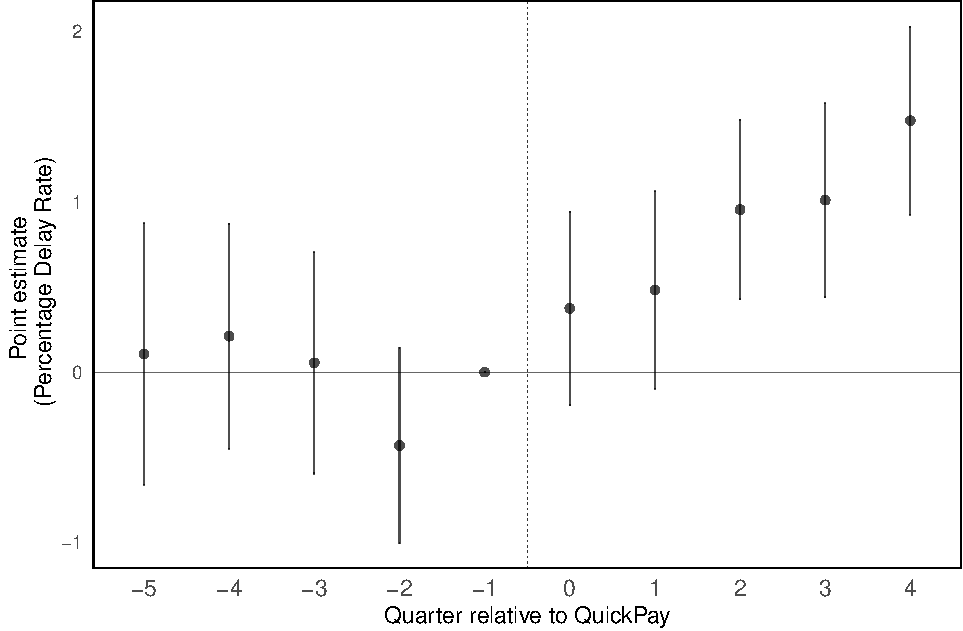
\includegraphics{qp_first_pc_delay-2_files/figure-latex/event_study-1.pdf}

\hypertarget{contract-financing}{%
\section{Contract Financing}\label{contract-financing}}

\[ CF_i = \begin{cases} 1, \text{ if project } i \text{ receives contract financing}\\
0, \text{ otherwise} \end{cases}\]

\[ \begin{aligned}
PercentDelay_{it} &=& \beta_0+\beta_1 Treat_i + \beta_2 Post_t + \beta_3 (Treat_i \times Post_t) \\
&+&\beta_4 CF_i + \beta_5 (CF_i \times Post_t) + \beta_6 (Treat_i \times Post_t \times CF_i) \\ 
&+&X_i + (Post_t \times X_i) + \mu_t + \theta_{firm} + \lambda_{task}+ \epsilon_{it}
\end{aligned}\]

\begin{table}[H] \centering 
  \caption{Financial constraints and QuickPay reform} 
  \label{} 
\small 
\begin{tabular}{@{\extracolsep{-2pt}}lccccc} 
\\[-1.8ex]\hline 
\hline \\[-1.8ex] 
\\[-1.8ex] & \multicolumn{5}{c}{$PercentDelay_{it}$  } \\ 
\\[-1.8ex] & (1) & (2) & (3) & (4) & (5)\\ 
\hline \\[-1.8ex] 
 $Treat_i$ & $-$4.73$^{***}$ & $-$3.19$^{***}$ & $-$3.22$^{***}$ & $-$2.42$^{***}$ & $-$2.44$^{***}$ \\ 
  & (0.22) & (0.18) & (0.18) & (0.18) & (0.18) \\ 
  & & & & & \\ 
 $Post_t$ & $-$1.60$^{***}$ & $-$19.78$^{***}$ &  &  &  \\ 
  & (0.22) & (1.52) &  &  &  \\ 
  & & & & & \\ 
 $Treat_i \times Post_t$ & 2.22$^{***}$ & 1.72$^{***}$ & 1.74$^{***}$ & 2.03$^{***}$ & 2.16$^{***}$ \\ 
  & (0.26) & (0.24) & (0.24) & (0.23) & (0.23) \\ 
  & & & & & \\ 
 $CF_i$ & 2.77$^{***}$ & 3.09$^{***}$ & 2.89$^{***}$ & $-$0.99$^{***}$ & $-$1.12$^{***}$ \\ 
  & (0.32) & (0.29) & (0.29) & (0.31) & (0.31) \\ 
  & & & & & \\ 
 $Post_t \times CF_i$ & $-$0.04 & $-$1.13$^{***}$ & $-$0.95$^{**}$ & 0.22 & 0.07 \\ 
  & (0.46) & (0.43) & (0.43) & (0.44) & (0.44) \\ 
  & & & & & \\ 
 $Post_t \times CF_i \times Treat_i$ & 3.35$^{***}$ & 2.08$^{***}$ & 2.14$^{***}$ & 0.75$^{*}$ & 0.85$^{**}$ \\ 
  & (0.48) & (0.41) & (0.41) & (0.43) & (0.43) \\ 
  & & & & & \\ 
 Constant & 10.66$^{***}$ & 97.94$^{***}$ &  &  &  \\ 
  & (0.19) & (1.15) &  &  &  \\ 
  & & & & & \\ 
\hline \\[-1.8ex] 
Duration, Budget, Bids & No & Yes & Yes & Yes & Yes \\ 
$Post_t \times $  (Duration, Budget, Bids) & No & Yes & Yes & Yes & Yes \\ 
Project stage & No & Yes & Yes & Yes & Yes \\ 
Year-Quarter fixed effects & No & No & Yes & Yes & Yes \\ 
Task fixed effects & No & No & No & Yes & Yes \\ 
Industry fixed effects & No & No & No & No & Yes \\ 
Observations & 260,056 & 235,960 & 235,960 & 235,960 & 235,960 \\ 
R$^{2}$ & 0.01 & 0.24 & 0.25 & 0.28 & 0.28 \\ 
Adjusted R$^{2}$ & 0.01 & 0.24 & 0.25 & 0.27 & 0.28 \\ 
\hline 
\hline \\[-1.8ex] 
\textit{Note:}  & \multicolumn{5}{r}{$^{*}$p$<$0.1; $^{**}$p$<$0.05; $^{***}$p$<$0.01} \\ 
 & \multicolumn{5}{r}{Each observation is a project-quarter.} \\ 
 & \multicolumn{5}{r}{SEs are robust and clustered at the project level.} \\ 
\end{tabular} 
\end{table}

\hypertarget{with-treat-x-cf-term}{%
\subsection{With Treat x CF term}\label{with-treat-x-cf-term}}

\begin{table}[H] \centering 
  \caption{Financial constraints and QuickPay reform} 
  \label{} 
\small 
\begin{tabular}{@{\extracolsep{-2pt}}lccccc} 
\\[-1.8ex]\hline 
\hline \\[-1.8ex] 
\\[-1.8ex] & \multicolumn{5}{c}{$PercentDelay_{it}$  } \\ 
\\[-1.8ex] & (1) & (2) & (3) & (4) & (5)\\ 
\hline \\[-1.8ex] 
 $Treat_i$ & $-$5.34$^{***}$ & $-$3.52$^{***}$ & $-$3.54$^{***}$ & $-$2.56$^{***}$ & $-$2.60$^{***}$ \\ 
  & (0.23) & (0.19) & (0.19) & (0.19) & (0.19) \\ 
  & & & & & \\ 
 $Post_t$ & $-$1.95$^{***}$ & $-$20.01$^{***}$ &  &  &  \\ 
  & (0.23) & (1.52) &  &  &  \\ 
  & & & & & \\ 
 $CF_i$ & 0.15 & 1.85$^{***}$ & 1.67$^{***}$ & $-$1.53$^{***}$ & $-$1.72$^{***}$ \\ 
  & (0.49) & (0.43) & (0.43) & (0.44) & (0.45) \\ 
  & & & & & \\ 
 $Treat_i \times Post_t$ & 2.84$^{***}$ & 2.05$^{***}$ & 2.06$^{***}$ & 2.17$^{***}$ & 2.31$^{***}$ \\ 
  & (0.28) & (0.25) & (0.25) & (0.24) & (0.24) \\ 
  & & & & & \\ 
 $Post_t \times CF_i$ & 2.57$^{***}$ & 0.11 & 0.26 & 0.73 & 0.64 \\ 
  & (0.59) & (0.54) & (0.54) & (0.54) & (0.54) \\ 
  & & & & & \\ 
 $Treat_i \times CF_i$ & 4.80$^{***}$ & 2.31$^{***}$ & 2.27$^{***}$ & 1.00$^{*}$ & 1.12$^{**}$ \\ 
  & (0.64) & (0.55) & (0.55) & (0.55) & (0.56) \\ 
  & & & & & \\ 
 $Treat_i \times Post_t \times CF_i$ & $-$1.45$^{*}$ & $-$0.23 & $-$0.13 & $-$0.21 & $-$0.22 \\ 
  & (0.79) & (0.71) & (0.71) & (0.71) & (0.71) \\ 
  & & & & & \\ 
 Constant & 11.01$^{***}$ & 98.17$^{***}$ &  &  &  \\ 
  & (0.20) & (1.15) &  &  &  \\ 
  & & & & & \\ 
\hline \\[-1.8ex] 
Duration, Budget, Bids & No & Yes & Yes & Yes & Yes \\ 
$Post_t \times $  (Duration, Budget, Bids) & No & Yes & Yes & Yes & Yes \\ 
Project stage & No & Yes & Yes & Yes & Yes \\ 
Year-Quarter fixed effects & No & No & Yes & Yes & Yes \\ 
Task fixed effects & No & No & No & Yes & Yes \\ 
Industry fixed effects & No & No & No & No & Yes \\ 
Observations & 260,056 & 235,960 & 235,960 & 235,960 & 235,960 \\ 
R$^{2}$ & 0.01 & 0.24 & 0.25 & 0.28 & 0.28 \\ 
Adjusted R$^{2}$ & 0.01 & 0.24 & 0.25 & 0.27 & 0.28 \\ 
\hline 
\hline \\[-1.8ex] 
\textit{Note:}  & \multicolumn{5}{r}{$^{*}$p$<$0.1; $^{**}$p$<$0.05; $^{***}$p$<$0.01} \\ 
 & \multicolumn{5}{r}{Each observation is a project-quarter.} \\ 
 & \multicolumn{5}{r}{SEs are robust and clustered at the project level.} \\ 
\end{tabular} 
\end{table}

\hypertarget{projects-active-onbefore-june-2010}{%
\subsection{Projects active on/before June
2010}\label{projects-active-onbefore-june-2010}}

\begin{itemize}
\tightlist
\item
  \(CF=1\) if project was receiving contract financing
\item
  Sample restricted to projects that started on or before June 2010
\item
  Jobs act was launched in Sept 2010
\end{itemize}

\begin{table}[H] \centering 
  \caption{Financial constraints and QuickPay reform} 
  \label{} 
\small 
\begin{tabular}{@{\extracolsep{-2pt}}lccccc} 
\\[-1.8ex]\hline 
\hline \\[-1.8ex] 
\\[-1.8ex] & \multicolumn{5}{c}{$PercentDelay_{it}$  } \\ 
\\[-1.8ex] & (1) & (2) & (3) & (4) & (5)\\ 
\hline \\[-1.8ex] 
 $Treat_i$ & $-$5.64$^{***}$ & $-$2.83$^{***}$ & $-$2.92$^{***}$ & $-$1.77$^{***}$ & $-$1.92$^{***}$ \\ 
  & (0.31) & (0.26) & (0.25) & (0.27) & (0.27) \\ 
  & & & & & \\ 
 $Post_t$ & $-$0.28 & $-$42.84$^{***}$ &  &  &  \\ 
  & (0.47) & (3.97) &  &  &  \\ 
  & & & & & \\ 
 $CF_i$ & $-$1.18$^{*}$ & 1.44$^{**}$ & 1.09$^{*}$ & $-$2.58$^{***}$ & $-$2.81$^{***}$ \\ 
  & (0.63) & (0.58) & (0.57) & (0.63) & (0.63) \\ 
  & & & & & \\ 
 $Treat_i \times Post_t$ & 1.13$^{**}$ & 4.82$^{***}$ & 4.85$^{***}$ & 4.88$^{***}$ & 4.95$^{***}$ \\ 
  & (0.57) & (0.76) & (0.75) & (0.80) & (0.80) \\ 
  & & & & & \\ 
 $Post_t \times CF_i$ & 1.65 & $-$0.12 & 0.22 & 2.69$^{**}$ & 2.79$^{**}$ \\ 
  & (1.11) & (1.16) & (1.15) & (1.21) & (1.21) \\ 
  & & & & & \\ 
 $Treat_i \times CF_i$ & 5.12$^{***}$ & 2.41$^{***}$ & 2.33$^{***}$ & 1.50$^{*}$ & 1.51$^{*}$ \\ 
  & (0.83) & (0.76) & (0.74) & (0.79) & (0.79) \\ 
  & & & & & \\ 
 $Treat_i \times Post_t \times CF_i$ & 1.01 & $-$2.58 & $-$2.43 & $-$1.76 & $-$2.05 \\ 
  & (1.58) & (1.64) & (1.63) & (1.69) & (1.69) \\ 
  & & & & & \\ 
 Constant & 11.65$^{***}$ & 103.65$^{***}$ &  &  &  \\ 
  & (0.27) & (1.57) &  &  &  \\ 
  & & & & & \\ 
\hline \\[-1.8ex] 
Duration, Budget, Bids & No & Yes & Yes & Yes & Yes \\ 
$Post_t \times $  (Duration, Budget, Bids) & No & Yes & Yes & Yes & Yes \\ 
Project stage & No & Yes & Yes & Yes & Yes \\ 
Year-Quarter fixed effects & No & No & Yes & Yes & Yes \\ 
Task fixed effects & No & No & No & Yes & Yes \\ 
Industry fixed effects & No & No & No & No & Yes \\ 
Observations & 75,119 & 64,292 & 64,292 & 64,292 & 64,292 \\ 
R$^{2}$ & 0.01 & 0.26 & 0.27 & 0.31 & 0.31 \\ 
Adjusted R$^{2}$ & 0.01 & 0.26 & 0.27 & 0.30 & 0.30 \\ 
\hline 
\hline \\[-1.8ex] 
\textit{Note:}  & \multicolumn{5}{r}{$^{*}$p$<$0.1; $^{**}$p$<$0.05; $^{***}$p$<$0.01} \\ 
 & \multicolumn{5}{r}{Each observation is a project-quarter.} \\ 
 & \multicolumn{5}{r}{SEs are robust and clustered at the project level.} \\ 
\end{tabular} 
\end{table}

\hypertarget{firm-level-financial-constraints-onbefore-june-2010}{%
\subsection{Firm level financial Constraints (on/before June
2010)}\label{firm-level-financial-constraints-onbefore-june-2010}}

\begin{itemize}
\tightlist
\item
  \(CF=1\) if contractor was receiving financing on any project prior on
  or before June 2010
\item
  Jobs act was launched in Sept 2010
\end{itemize}

\begin{table}[H] \centering 
  \caption{Financial constraints and QuickPay reform} 
  \label{} 
\small 
\begin{tabular}{@{\extracolsep{-2pt}}lccccc} 
\\[-1.8ex]\hline 
\hline \\[-1.8ex] 
\\[-1.8ex] & \multicolumn{5}{c}{$PercentDelay_{it}$  } \\ 
\\[-1.8ex] & (1) & (2) & (3) & (4) & (5)\\ 
\hline \\[-1.8ex] 
 $Treat_i$ & $-$0.56$^{**}$ & $-$0.75$^{***}$ & $-$0.82$^{***}$ & $-$1.19$^{***}$ & $-$1.23$^{***}$ \\ 
  & (0.25) & (0.24) & (0.24) & (0.24) & (0.24) \\ 
  & & & & & \\ 
 $Post_t$ & $-$0.30 & $-$19.58$^{***}$ &  &  &  \\ 
  & (0.24) & (1.59) &  &  &  \\ 
  & & & & & \\ 
 $CF_i$ & 8.74$^{***}$ & 5.73$^{***}$ & 5.54$^{***}$ & 2.14$^{***}$ & 2.18$^{***}$ \\ 
  & (0.37) & (0.27) & (0.27) & (0.28) & (0.29) \\ 
  & & & & & \\ 
 $Treat_i \times Post_t$ & 0.52$^{*}$ & $-$0.08 & $-$0.04 & 0.88$^{***}$ & 1.13$^{***}$ \\ 
  & (0.31) & (0.30) & (0.30) & (0.30) & (0.30) \\ 
  & & & & & \\ 
 $Post_t \times CF_i$ & $-$2.85$^{***}$ & $-$3.41$^{***}$ & $-$3.25$^{***}$ & $-$2.37$^{***}$ & $-$2.28$^{***}$ \\ 
  & (0.43) & (0.35) & (0.35) & (0.35) & (0.35) \\ 
  & & & & & \\ 
 $Treat_i \times CF_i$ & $-$8.41$^{***}$ & $-$4.60$^{***}$ & $-$4.48$^{***}$ & $-$2.41$^{***}$ & $-$2.42$^{***}$ \\ 
  & (0.44) & (0.36) & (0.36) & (0.36) & (0.36) \\ 
  & & & & & \\ 
 $Treat_i \times Post_t \times CF_i$ & 3.73$^{***}$ & 3.47$^{***}$ & 3.38$^{***}$ & 2.22$^{***}$ & 2.07$^{***}$ \\ 
  & (0.53) & (0.46) & (0.46) & (0.46) & (0.46) \\ 
  & & & & & \\ 
 Constant & 6.54$^{***}$ & 93.96$^{***}$ &  &  &  \\ 
  & (0.20) & (1.19) &  &  &  \\ 
  & & & & & \\ 
\hline \\[-1.8ex] 
Duration, Budget, Bids & No & Yes & Yes & Yes & Yes \\ 
$Post_t \times $  (Duration, Budget, Bids) & No & Yes & Yes & Yes & Yes \\ 
Project stage & No & Yes & Yes & Yes & Yes \\ 
Year-Quarter fixed effects & No & No & Yes & Yes & Yes \\ 
Task fixed effects & No & No & No & Yes & Yes \\ 
Industry fixed effects & No & No & No & No & Yes \\ 
Observations & 229,552 & 209,046 & 209,046 & 209,046 & 209,046 \\ 
R$^{2}$ & 0.01 & 0.25 & 0.25 & 0.28 & 0.29 \\ 
Adjusted R$^{2}$ & 0.01 & 0.25 & 0.25 & 0.28 & 0.28 \\ 
\hline 
\hline \\[-1.8ex] 
\textit{Note:}  & \multicolumn{5}{r}{$^{*}$p$<$0.1; $^{**}$p$<$0.05; $^{***}$p$<$0.01} \\ 
 & \multicolumn{5}{r}{Each observation is a project-quarter.} \\ 
 & \multicolumn{5}{r}{SEs are robust and clustered at the project level.} \\ 
\end{tabular} 
\end{table}

\hypertarget{plots}{%
\subsection{Plots}\label{plots}}

\begin{verbatim}
## Warning: Removed 255008 rows containing non-finite values (stat_density).
\end{verbatim}

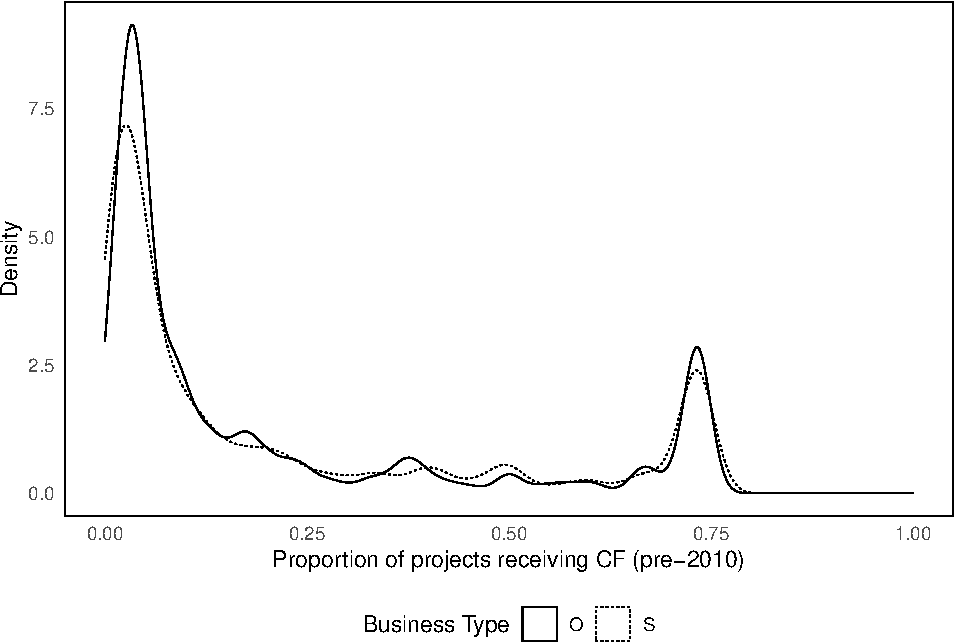
\includegraphics{qp_first_pc_delay-2_files/figure-latex/cf_plots-1.pdf}

\hypertarget{receives-grantsfinancial-assistance}{%
\section{Receives Grants/Financial
Assistance}\label{receives-grantsfinancial-assistance}}

\begin{itemize}
\tightlist
\item
  \(CF=1\) if receives\_grants==`t'
\item
  The variable ``receives\_grants'' used to be called ``receives
  financial assistance''
\end{itemize}

\hypertarget{all-projects}{%
\subsection{All projects}\label{all-projects}}

\begin{table}[H] \centering 
  \caption{Financial constraints and QuickPay reform} 
  \label{} 
\small 
\begin{tabular}{@{\extracolsep{-2pt}}lccccc} 
\\[-1.8ex]\hline 
\hline \\[-1.8ex] 
\\[-1.8ex] & \multicolumn{5}{c}{$PercentDelay_{it}$  } \\ 
\\[-1.8ex] & (1) & (2) & (3) & (4) & (5)\\ 
\hline \\[-1.8ex] 
 $Treat_i$ & $-$3.57$^{***}$ & $-$2.88$^{***}$ & $-$2.89$^{***}$ & $-$2.09$^{***}$ & $-$2.12$^{***}$ \\ 
  & (0.21) & (0.19) & (0.19) & (0.19) & (0.19) \\ 
  & & & & & \\ 
 $Post_t$ & $-$0.83$^{***}$ & $-$20.40$^{***}$ &  &  &  \\ 
  & (0.21) & (1.58) &  &  &  \\ 
  & & & & & \\ 
 $CF_i$ & 27.38$^{***}$ & 10.71$^{***}$ & 10.52$^{***}$ & 8.51$^{***}$ & 8.72$^{***}$ \\ 
  & (1.54) & (0.83) & (0.83) & (0.84) & (0.84) \\ 
  & & & & & \\ 
 $Treat_i \times Post_t$ & 1.48$^{***}$ & 1.38$^{***}$ & 1.39$^{***}$ & 1.67$^{***}$ & 1.86$^{***}$ \\ 
  & (0.26) & (0.24) & (0.24) & (0.24) & (0.24) \\ 
  & & & & & \\ 
 $Post_t \times CF_i$ & $-$18.78$^{***}$ & $-$8.51$^{***}$ & $-$8.37$^{***}$ & $-$8.03$^{***}$ & $-$7.74$^{***}$ \\ 
  & (1.64) & (1.03) & (1.03) & (1.03) & (1.04) \\ 
  & & & & & \\ 
 $Treat_i \times CF_i$ & $-$21.05$^{***}$ & $-$4.21$^{***}$ & $-$4.04$^{***}$ & $-$4.66$^{***}$ & $-$4.94$^{***}$ \\ 
  & (1.80) & (1.17) & (1.17) & (1.17) & (1.18) \\ 
  & & & & & \\ 
 $Treat_i \times Post_t \times CF_i$ & 16.60$^{***}$ & 5.98$^{***}$ & 5.82$^{***}$ & 6.45$^{***}$ & 6.16$^{***}$ \\ 
  & (1.97) & (1.48) & (1.48) & (1.48) & (1.48) \\ 
  & & & & & \\ 
 Constant & 9.48$^{***}$ & 95.63$^{***}$ &  &  &  \\ 
  & (0.17) & (1.18) &  &  &  \\ 
  & & & & & \\ 
\hline \\[-1.8ex] 
Duration, Budget, Bids & No & Yes & Yes & Yes & Yes \\ 
$Post_t \times $  (Duration, Budget, Bids) & No & Yes & Yes & Yes & Yes \\ 
Project stage & No & Yes & Yes & Yes & Yes \\ 
Year-Quarter fixed effects & No & No & Yes & Yes & Yes \\ 
Task fixed effects & No & No & No & Yes & Yes \\ 
Industry fixed effects & No & No & No & No & Yes \\ 
Observations & 229,552 & 209,046 & 209,046 & 209,046 & 209,046 \\ 
R$^{2}$ & 0.01 & 0.25 & 0.25 & 0.29 & 0.29 \\ 
Adjusted R$^{2}$ & 0.01 & 0.25 & 0.25 & 0.28 & 0.28 \\ 
\hline 
\hline \\[-1.8ex] 
\textit{Note:}  & \multicolumn{5}{r}{$^{*}$p$<$0.1; $^{**}$p$<$0.05; $^{***}$p$<$0.01} \\ 
 & \multicolumn{5}{r}{Each observation is a project-quarter.} \\ 
 & \multicolumn{5}{r}{SEs are robust and clustered at the project level.} \\ 
\end{tabular} 
\end{table}

\hypertarget{projects-active-onbefore-june-2010-1}{%
\subsection{Projects active on/before June
2010}\label{projects-active-onbefore-june-2010-1}}

\begin{table}[H] \centering 
  \caption{Financial constraints and QuickPay reform} 
  \label{} 
\small 
\begin{tabular}{@{\extracolsep{-2pt}}lccccc} 
\\[-1.8ex]\hline 
\hline \\[-1.8ex] 
\\[-1.8ex] & \multicolumn{5}{c}{$PercentDelay_{it}$  } \\ 
\\[-1.8ex] & (1) & (2) & (3) & (4) & (5)\\ 
\hline \\[-1.8ex] 
 $Treat_i$ & $-$3.68$^{***}$ & $-$2.12$^{***}$ & $-$2.26$^{***}$ & $-$1.25$^{***}$ & $-$1.39$^{***}$ \\ 
  & (0.27) & (0.25) & (0.24) & (0.26) & (0.26) \\ 
  & & & & & \\ 
 $Post_t$ & 0.94$^{**}$ & $-$39.04$^{***}$ &  &  &  \\ 
  & (0.42) & (3.90) &  &  &  \\ 
  & & & & & \\ 
 $CF_i$ & 29.22$^{***}$ & 11.41$^{***}$ & 10.39$^{***}$ & 8.09$^{***}$ & 8.38$^{***}$ \\ 
  & (2.10) & (1.11) & (1.10) & (1.14) & (1.13) \\ 
  & & & & & \\ 
 $Treat_i \times Post_t$ & 0.43 & 3.69$^{***}$ & 3.79$^{***}$ & 3.92$^{***}$ & 3.88$^{***}$ \\ 
  & (0.53) & (0.68) & (0.68) & (0.72) & (0.73) \\ 
  & & & & & \\ 
 $Post_t \times CF_i$ & $-$21.69$^{***}$ & $-$14.54$^{***}$ & $-$13.38$^{***}$ & $-$10.20$^{***}$ & $-$10.19$^{***}$ \\ 
  & (2.56) & (2.37) & (2.35) & (2.39) & (2.37) \\ 
  & & & & & \\ 
 $Treat_i \times CF_i$ & $-$23.02$^{***}$ & $-$4.65$^{***}$ & $-$3.89$^{***}$ & $-$4.88$^{***}$ & $-$5.26$^{***}$ \\ 
  & (2.37) & (1.50) & (1.49) & (1.50) & (1.50) \\ 
  & & & & & \\ 
 $Treat_i \times Post_t \times CF_i$ & 18.56$^{***}$ & 10.02$^{***}$ & 9.30$^{***}$ & 9.13$^{***}$ & 9.52$^{***}$ \\ 
  & (3.07) & (3.36) & (3.34) & (3.37) & (3.35) \\ 
  & & & & & \\ 
 Constant & 9.87$^{***}$ & 100.44$^{***}$ &  &  &  \\ 
  & (0.22) & (1.55) &  &  &  \\ 
  & & & & & \\ 
\hline \\[-1.8ex] 
Duration, Budget, Bids & No & Yes & Yes & Yes & Yes \\ 
$Post_t \times $  (Duration, Budget, Bids) & No & Yes & Yes & Yes & Yes \\ 
Project stage & No & Yes & Yes & Yes & Yes \\ 
Year-Quarter fixed effects & No & No & Yes & Yes & Yes \\ 
Task fixed effects & No & No & No & Yes & Yes \\ 
Industry fixed effects & No & No & No & No & Yes \\ 
Observations & 74,942 & 64,129 & 64,129 & 64,129 & 64,129 \\ 
R$^{2}$ & 0.02 & 0.27 & 0.27 & 0.31 & 0.31 \\ 
Adjusted R$^{2}$ & 0.02 & 0.27 & 0.27 & 0.30 & 0.30 \\ 
\hline 
\hline \\[-1.8ex] 
\textit{Note:}  & \multicolumn{5}{r}{$^{*}$p$<$0.1; $^{**}$p$<$0.05; $^{***}$p$<$0.01} \\ 
 & \multicolumn{5}{r}{Each observation is a project-quarter.} \\ 
 & \multicolumn{5}{r}{SEs are robust and clustered at the project level.} \\ 
\end{tabular} 
\end{table}

\hypertarget{firm-level-financial-constraints-onbefore-june-2010-1}{%
\subsection{Firm level financial constraints (on/before June
2010)}\label{firm-level-financial-constraints-onbefore-june-2010-1}}

\begin{table}[H] \centering 
  \caption{Financial constraints and QuickPay reform} 
  \label{} 
\small 
\begin{tabular}{@{\extracolsep{-2pt}}lccccc} 
\\[-1.8ex]\hline 
\hline \\[-1.8ex] 
\\[-1.8ex] & \multicolumn{5}{c}{$PercentDelay_{it}$  } \\ 
\\[-1.8ex] & (1) & (2) & (3) & (4) & (5)\\ 
\hline \\[-1.8ex] 
 $Treat_i$ & $-$2.37$^{***}$ & $-$2.32$^{***}$ & $-$2.35$^{***}$ & $-$1.59$^{***}$ & $-$1.61$^{***}$ \\ 
  & (0.21) & (0.20) & (0.20) & (0.19) & (0.20) \\ 
  & & & & & \\ 
 $Post_t$ & $-$0.98$^{***}$ & $-$20.93$^{***}$ &  &  &  \\ 
  & (0.20) & (1.57) &  &  &  \\ 
  & & & & & \\ 
 $CF_i$ & 18.23$^{***}$ & 7.16$^{***}$ & 7.00$^{***}$ & 5.75$^{***}$ & 5.90$^{***}$ \\ 
  & (0.82) & (0.45) & (0.45) & (0.46) & (0.46) \\ 
  & & & & & \\ 
 $Treat_i \times Post_t$ & 1.61$^{***}$ & 1.38$^{***}$ & 1.39$^{***}$ & 1.60$^{***}$ & 1.82$^{***}$ \\ 
  & (0.25) & (0.25) & (0.25) & (0.25) & (0.25) \\ 
  & & & & & \\ 
 $Post_t \times CF_i$ & $-$6.82$^{***}$ & $-$3.37$^{***}$ & $-$3.24$^{***}$ & $-$3.55$^{***}$ & $-$3.33$^{***}$ \\ 
  & (0.93) & (0.59) & (0.59) & (0.58) & (0.58) \\ 
  & & & & & \\ 
 $Treat_i \times CF_i$ & $-$15.77$^{***}$ & $-$5.06$^{***}$ & $-$4.94$^{***}$ & $-$4.56$^{***}$ & $-$4.64$^{***}$ \\ 
  & (0.99) & (0.68) & (0.68) & (0.66) & (0.67) \\ 
  & & & & & \\ 
 $Treat_i \times Post_t \times CF_i$ & 6.11$^{***}$ & 2.47$^{***}$ & 2.38$^{***}$ & 2.83$^{***}$ & 2.57$^{***}$ \\ 
  & (1.15) & (0.89) & (0.89) & (0.88) & (0.88) \\ 
  & & & & & \\ 
 Constant & 8.33$^{***}$ & 94.90$^{***}$ &  &  &  \\ 
  & (0.17) & (1.18) &  &  &  \\ 
  & & & & & \\ 
\hline \\[-1.8ex] 
Duration, Budget, Bids & No & Yes & Yes & Yes & Yes \\ 
$Post_t \times $  (Duration, Budget, Bids) & No & Yes & Yes & Yes & Yes \\ 
Project stage & No & Yes & Yes & Yes & Yes \\ 
Year-Quarter fixed effects & No & No & Yes & Yes & Yes \\ 
Task fixed effects & No & No & No & Yes & Yes \\ 
Industry fixed effects & No & No & No & No & Yes \\ 
Observations & 229,552 & 209,046 & 209,046 & 209,046 & 209,046 \\ 
R$^{2}$ & 0.02 & 0.25 & 0.25 & 0.29 & 0.29 \\ 
Adjusted R$^{2}$ & 0.02 & 0.25 & 0.25 & 0.28 & 0.28 \\ 
\hline 
\hline \\[-1.8ex] 
\textit{Note:}  & \multicolumn{5}{r}{$^{*}$p$<$0.1; $^{**}$p$<$0.05; $^{***}$p$<$0.01} \\ 
 & \multicolumn{5}{r}{Each observation is a project-quarter.} \\ 
 & \multicolumn{5}{r}{SEs are robust and clustered at the project level.} \\ 
\end{tabular} 
\end{table}

\hypertarget{plots-1}{%
\subsection{Plots}\label{plots-1}}

\begin{verbatim}
## Warning: Removed 394825 rows containing non-finite values (stat_density).
\end{verbatim}

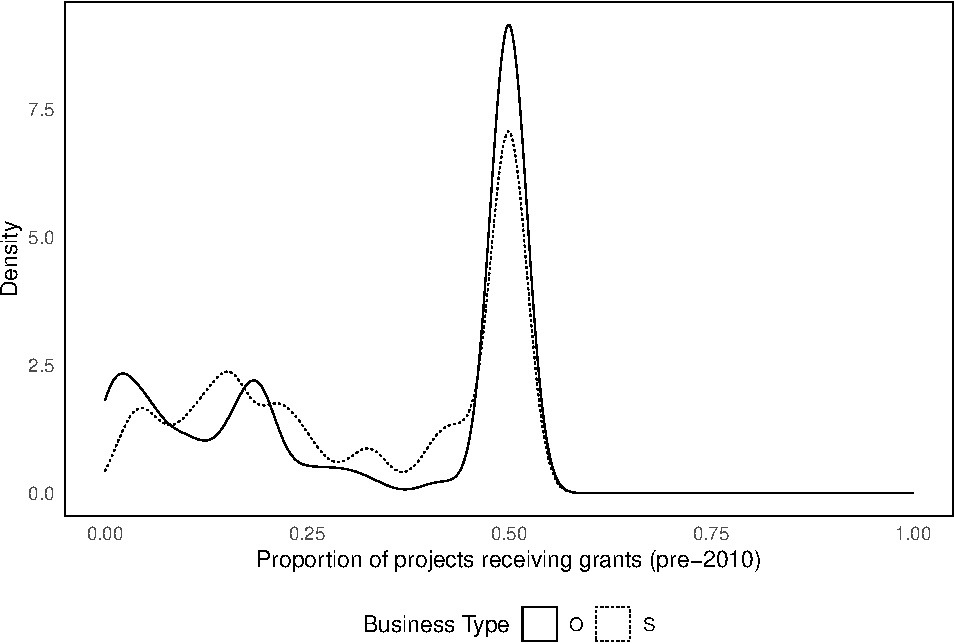
\includegraphics{qp_first_pc_delay-2_files/figure-latex/grants_plots-1.pdf}

\hypertarget{competition}{%
\section{Competition}\label{competition}}

\hypertarget{impact-on-bidding-metrics}{%
\subsection{Impact on bidding metrics}\label{impact-on-bidding-metrics}}

\begin{table}[H] \centering 
  \caption{Effect of Competition After QuickPay: Quickpay 2009-2011} 
  \label{} 
\small 
\begin{tabular}{@{\extracolsep{0pt}}lccc} 
\\[-1.8ex]\hline 
\hline \\[-1.8ex] 
\\[-1.8ex] & $NumberOfBids_{it}$ & $InitialDuration_{it}$ & $InitialBudget_{it}$ \\ 
\\[-1.8ex] & (1) & (2) & (3)\\ 
\hline \\[-1.8ex] 
 $Treat_i$ & 1.16$^{***}$ & $-$11.19$^{***}$ & $-$67,228.67$^{***}$ \\ 
  & (0.09) & (0.79) & (5,127.43) \\ 
  & & & \\ 
 $Treat_i \times Post_t$ & 0.14 & $-$1.70 & $-$28,346.23$^{***}$ \\ 
  & (0.13) & (1.09) & (7,219.64) \\ 
  & & & \\ 
\hline \\[-1.8ex] 
Task fixed effects & Yes & Yes & Yes \\ 
Time fixed effects & Yes & Yes & Yes \\ 
Observations & 203,106 & 198,967 & 203,144 \\ 
R$^{2}$ & 0.34 & 0.23 & 0.24 \\ 
Adjusted R$^{2}$ & 0.33 & 0.23 & 0.23 \\ 
\hline 
\hline \\[-1.8ex] 
\textit{Note:}  & \multicolumn{3}{r}{$^{*}$p$<$0.1; $^{**}$p$<$0.05; $^{***}$p$<$0.01} \\ 
 & \multicolumn{3}{r}{Each observation is a project-quarter.} \\ 
 & \multicolumn{3}{r}{SEs are robust and clustered at the project level.} \\ 
 & \multicolumn{3}{r}{Sample restricted to fully competed projects.} \\ 
\end{tabular} 
\end{table}

\hypertarget{impact-on-delays}{%
\subsection{Impact on delays}\label{impact-on-delays}}

Define
\[ SA_i = \begin{cases} 1, \text{ if project was signed after QuickPay}\\
0, \text{ otherwise} \end{cases}\]

\[ SB_i = \begin{cases} 1, \text{ if project was signed before QuickPay}\\
0, \text{ otherwise} \end{cases}\]

\hypertarget{subsample-model}{%
\subsubsection{Subsample model}\label{subsample-model}}

For a subsample of competitive or noncompetitive projects:

\[ \begin{aligned} PercentDelay_{it} &=& \beta_0 +\beta_1 Treat_i+ \beta_2 SA_i+ \beta_3 Post_t \\&+& \beta_4 (Treat_i \times Post_t \times SA_i )+\beta_5 (Treat_i \times Post_t \times SB_i )+e_{it} \end{aligned} \]

\begin{itemize}
\item
  According to our hypothesis, \(\beta_4\) should be positive and
  significant for competitive projects, and insignificant for
  non-competitive projects.
\item
  In the following regressions, we also control for the project's age.
  Project's age is defined as the number of quarters since it first
  showed up in the sample. We include the terciles of project's age as a
  control variable.
\end{itemize}

\begin{table}[H] \centering 
  \caption{Effect of QuickPay on competitively awarded projects} 
  \label{} 
\small 
\begin{tabular}{@{\extracolsep{-2pt}}lccccc} 
\\[-1.8ex]\hline 
\hline \\[-1.8ex] 
\\[-1.8ex] & \multicolumn{5}{c}{$PercentDelay_{it}$  } \\ 
\\[-1.8ex] & (1) & (2) & (3) & (4) & (5)\\ 
\hline \\[-1.8ex] 
 $Treat_i$ & $-$6.09$^{***}$ & $-$5.53$^{***}$ & $-$5.53$^{***}$ & $-$3.34$^{***}$ & $-$3.34$^{***}$ \\ 
  & (0.25) & (0.24) & (0.24) & (0.24) & (0.24) \\ 
  & & & & & \\ 
 $SA_i$ & $-$2.40$^{***}$ & 2.48$^{***}$ & 4.06$^{***}$ & 4.63$^{***}$ & 4.52$^{***}$ \\ 
  & (0.31) & (0.31) & (0.33) & (0.33) & (0.33) \\ 
  & & & & & \\ 
 $Post_t$ & $-$0.08 & $-$4.18$^{***}$ &  &  &  \\ 
  & (0.29) & (0.30) &  &  &  \\ 
  & & & & & \\ 
 $Treat_i \times SB_i \times Post_t$ & 1.46$^{***}$ & 1.62$^{***}$ & 1.63$^{***}$ & 2.09$^{***}$ & 2.15$^{***}$ \\ 
  & (0.35) & (0.34) & (0.34) & (0.33) & (0.33) \\ 
  & & & & & \\ 
 $Treat_i \times SA_i \times Post_t$ & 2.50$^{***}$ & 2.03$^{***}$ & 2.02$^{***}$ & 2.30$^{***}$ & 2.43$^{***}$ \\ 
  & (0.36) & (0.34) & (0.34) & (0.33) & (0.33) \\ 
  & & & & & \\ 
 Constant & 11.71$^{***}$ & 19.48$^{***}$ &  &  &  \\ 
  & (0.22) & (0.26) &  &  &  \\ 
  & & & & & \\ 
\hline \\[-1.8ex] 
Project stage & No & Yes & Yes & Yes & Yes \\ 
Year-Quarter fixed effects & No & No & Yes & Yes & Yes \\ 
Task fixed effects & No & No & No & Yes & Yes \\ 
Industry fixed effects & No & No & No & No & Yes \\ 
Observations & 188,945 & 188,901 & 188,901 & 188,901 & 188,901 \\ 
R$^{2}$ & 0.01 & 0.05 & 0.06 & 0.13 & 0.14 \\ 
Adjusted R$^{2}$ & 0.01 & 0.05 & 0.06 & 0.13 & 0.13 \\ 
\hline 
\hline \\[-1.8ex] 
\textit{Note:}  & \multicolumn{5}{r}{$^{*}$p$<$0.1; $^{**}$p$<$0.05; $^{***}$p$<$0.01} \\ 
 & \multicolumn{5}{r}{Each observation is a project-quarter.} \\ 
 & \multicolumn{5}{r}{SEs are robust and clustered at the project level.} \\ 
 & \multicolumn{5}{r}{Sample restricted to fully competed projects.} \\ 
\end{tabular} 
\end{table}

\begin{table}[H] \centering 
  \caption{Effect of QuickPay on non-competitively awarded projects} 
  \label{} 
\small 
\begin{tabular}{@{\extracolsep{-2pt}}lccccc} 
\\[-1.8ex]\hline 
\hline \\[-1.8ex] 
\\[-1.8ex] & \multicolumn{5}{c}{$PercentDelay_{it}$  } \\ 
\\[-1.8ex] & (1) & (2) & (3) & (4) & (5)\\ 
\hline \\[-1.8ex] 
 $Treat_i$ & 1.69$^{***}$ & 1.57$^{***}$ & 1.42$^{***}$ & $-$0.61 & $-$0.26 \\ 
  & (0.54) & (0.52) & (0.52) & (0.55) & (0.55) \\ 
  & & & & & \\ 
 $SA_i$ & $-$0.61 & 3.48$^{***}$ & 5.89$^{***}$ & 5.05$^{***}$ & 5.03$^{***}$ \\ 
  & (0.40) & (0.40) & (0.49) & (0.51) & (0.51) \\ 
  & & & & & \\ 
 $Post_t$ & $-$1.76$^{***}$ & $-$5.44$^{***}$ &  &  &  \\ 
  & (0.44) & (0.45) &  &  &  \\ 
  & & & & & \\ 
 $Treat_i \times SB_i \times Post_t$ & 2.87$^{***}$ & 2.48$^{***}$ & 2.41$^{***}$ & 1.85$^{**}$ & 1.72$^{**}$ \\ 
  & (0.78) & (0.75) & (0.76) & (0.76) & (0.77) \\ 
  & & & & & \\ 
 $Treat_i \times SA_i \times Post_t$ & 1.01 & 0.87 & 0.80 & 0.03 & 0.04 \\ 
  & (0.78) & (0.74) & (0.75) & (0.75) & (0.75) \\ 
  & & & & & \\ 
 Constant & 8.10$^{***}$ & 16.34$^{***}$ &  &  &  \\ 
  & (0.35) & (0.46) &  &  &  \\ 
  & & & & & \\ 
\hline \\[-1.8ex] 
Project stage & No & Yes & Yes & Yes & Yes \\ 
Year-Quarter fixed effects & No & No & Yes & Yes & Yes \\ 
Task fixed effects & No & No & No & Yes & Yes \\ 
Industry fixed effects & No & No & No & No & Yes \\ 
Observations & 40,464 & 40,456 & 40,456 & 40,456 & 40,456 \\ 
R$^{2}$ & 0.004 & 0.05 & 0.05 & 0.12 & 0.13 \\ 
Adjusted R$^{2}$ & 0.003 & 0.05 & 0.05 & 0.11 & 0.11 \\ 
\hline 
\hline \\[-1.8ex] 
\textit{Note:}  & \multicolumn{5}{r}{$^{*}$p$<$0.1; $^{**}$p$<$0.05; $^{***}$p$<$0.01} \\ 
 & \multicolumn{5}{r}{Each observation is a project-quarter.} \\ 
 & \multicolumn{5}{r}{SEs are robust and clustered at the project level.} \\ 
 & \multicolumn{5}{r}{Sample restricted to non-competed projects.} \\ 
\end{tabular} 
\end{table}

\hypertarget{subsample-model-ii}{%
\subsubsection{Subsample model II}\label{subsample-model-ii}}

\begin{table}[H] \centering 
  \caption{Effect of QuickPay on competitively awarded projects} 
  \label{} 
\small 
\begin{tabular}{@{\extracolsep{-2pt}}lccccc} 
\\[-1.8ex]\hline 
\hline \\[-1.8ex] 
\\[-1.8ex] & \multicolumn{5}{c}{$PercentDelay_{it}$  } \\ 
\\[-1.8ex] & (1) & (2) & (3) & (4) & (5)\\ 
\hline \\[-1.8ex] 
 $Treat_i$ & $-$6.09$^{***}$ & $-$5.53$^{***}$ & $-$5.53$^{***}$ & $-$3.34$^{***}$ & $-$3.34$^{***}$ \\ 
  & (0.25) & (0.24) & (0.24) & (0.24) & (0.24) \\ 
  & & & & & \\ 
 $SA_i$ & $-$2.40$^{***}$ & 2.48$^{***}$ & 4.06$^{***}$ & 4.63$^{***}$ & 4.52$^{***}$ \\ 
  & (0.31) & (0.31) & (0.33) & (0.33) & (0.33) \\ 
  & & & & & \\ 
 $Post_t$ & $-$0.08 & $-$4.18$^{***}$ &  &  &  \\ 
  & (0.29) & (0.30) &  &  &  \\ 
  & & & & & \\ 
 $Treat_i \times Post_t$ & 1.46$^{***}$ & 1.62$^{***}$ & 1.63$^{***}$ & 2.09$^{***}$ & 2.15$^{***}$ \\ 
  & (0.35) & (0.34) & (0.34) & (0.33) & (0.33) \\ 
  & & & & & \\ 
 $Treat_i \times Post_t \times SA_i $ & 1.04$^{***}$ & 0.41 & 0.38 & 0.21 & 0.28 \\ 
  & (0.37) & (0.35) & (0.35) & (0.35) & (0.35) \\ 
  & & & & & \\ 
 Constant & 11.71$^{***}$ & 19.48$^{***}$ &  &  &  \\ 
  & (0.22) & (0.26) &  &  &  \\ 
  & & & & & \\ 
\hline \\[-1.8ex] 
Project stage & No & Yes & Yes & Yes & Yes \\ 
Year-Quarter fixed effects & No & No & Yes & Yes & Yes \\ 
Task fixed effects & No & No & No & Yes & Yes \\ 
Industry fixed effects & No & No & No & No & Yes \\ 
Observations & 188,945 & 188,901 & 188,901 & 188,901 & 188,901 \\ 
R$^{2}$ & 0.01 & 0.05 & 0.06 & 0.13 & 0.14 \\ 
Adjusted R$^{2}$ & 0.01 & 0.05 & 0.06 & 0.13 & 0.13 \\ 
\hline 
\hline \\[-1.8ex] 
\textit{Note:}  & \multicolumn{5}{r}{$^{*}$p$<$0.1; $^{**}$p$<$0.05; $^{***}$p$<$0.01} \\ 
 & \multicolumn{5}{r}{Each observation is a project-quarter.} \\ 
 & \multicolumn{5}{r}{SEs are robust and clustered at the project level.} \\ 
 & \multicolumn{5}{r}{Sample restricted to fully competed projects.} \\ 
\end{tabular} 
\end{table}

\begin{table}[H] \centering 
  \caption{Effect of QuickPay on non-competitively awarded projects} 
  \label{} 
\small 
\begin{tabular}{@{\extracolsep{-2pt}}lccccc} 
\\[-1.8ex]\hline 
\hline \\[-1.8ex] 
\\[-1.8ex] & \multicolumn{5}{c}{$PercentDelay_{it}$  } \\ 
\\[-1.8ex] & (1) & (2) & (3) & (4) & (5)\\ 
\hline \\[-1.8ex] 
 $Treat_i$ & 1.69$^{***}$ & 1.57$^{***}$ & 1.42$^{***}$ & $-$0.61 & $-$0.26 \\ 
  & (0.54) & (0.52) & (0.52) & (0.55) & (0.55) \\ 
  & & & & & \\ 
 $SA_i$ & $-$0.61 & 3.48$^{***}$ & 5.89$^{***}$ & 5.05$^{***}$ & 5.03$^{***}$ \\ 
  & (0.40) & (0.40) & (0.49) & (0.51) & (0.51) \\ 
  & & & & & \\ 
 $Post_t$ & $-$1.76$^{***}$ & $-$5.44$^{***}$ &  &  &  \\ 
  & (0.44) & (0.45) &  &  &  \\ 
  & & & & & \\ 
 $Treat_i \times Post_t$ & 2.87$^{***}$ & 2.48$^{***}$ & 2.41$^{***}$ & 1.85$^{**}$ & 1.72$^{**}$ \\ 
  & (0.78) & (0.75) & (0.76) & (0.76) & (0.77) \\ 
  & & & & & \\ 
 $Treat_i \times Post_t \times SA_i $ & $-$1.86$^{**}$ & $-$1.61$^{**}$ & $-$1.61$^{**}$ & $-$1.82$^{**}$ & $-$1.68$^{**}$ \\ 
  & (0.80) & (0.75) & (0.76) & (0.77) & (0.77) \\ 
  & & & & & \\ 
 Constant & 8.10$^{***}$ & 16.34$^{***}$ &  &  &  \\ 
  & (0.35) & (0.46) &  &  &  \\ 
  & & & & & \\ 
\hline \\[-1.8ex] 
Project stage & No & Yes & Yes & Yes & Yes \\ 
Year-Quarter fixed effects & No & No & Yes & Yes & Yes \\ 
Task fixed effects & No & No & No & Yes & Yes \\ 
Industry fixed effects & No & No & No & No & Yes \\ 
Observations & 40,464 & 40,456 & 40,456 & 40,456 & 40,456 \\ 
R$^{2}$ & 0.004 & 0.05 & 0.05 & 0.12 & 0.13 \\ 
Adjusted R$^{2}$ & 0.003 & 0.05 & 0.05 & 0.11 & 0.11 \\ 
\hline 
\hline \\[-1.8ex] 
\textit{Note:}  & \multicolumn{5}{r}{$^{*}$p$<$0.1; $^{**}$p$<$0.05; $^{***}$p$<$0.01} \\ 
 & \multicolumn{5}{r}{Each observation is a project-quarter.} \\ 
 & \multicolumn{5}{r}{SEs are robust and clustered at the project level.} \\ 
 & \multicolumn{5}{r}{Sample restricted to non-competed projects.} \\ 
\end{tabular} 
\end{table}

\hypertarget{four-way-interaction}{%
\subsubsection{Four-way interaction}\label{four-way-interaction}}

We run the following model:

\[\begin{aligned} PercentDelay_{it} &=& \beta_0 +\beta_1 Treat_i+ \beta_2 StartedAfterQP_i+ \beta_3 Post_t+ \beta_4 Competitive_i\\ && +  \beta_5 (Treat_i \times Competitive_i) + \beta_6 (Post_t \times Competitive_i)\\ && +  \beta_7 (StartedAfterQP_i \times Competitive_i) +\beta_8 (Treat_i \times Post_t)\\ && + \beta_9 (Treat_i \times Post_t \times Competitive_i) \\ && + \beta_{10} (Treat_i \times Post_t \times StartedAfterQP_i )\\ && + \beta_{11} (Treat_i \times Post_t \times StartedAfterQP_i \times Competitive_i) + e_{it} \end{aligned}\]

\textbf{Interpretation:}

\begin{itemize}
\tightlist
\item
  \(\beta_9\) is the difference between treatment effect for competitive
  and non-competitive projects signed before quickpay.
\item
  \(\beta_9 + \beta_{11}\) is the difference between treatment effect
  for competitive and non-competitive projects signed \emph{after}
  quickpay.
\item
  \(\beta_{11}\) is our coefficient of interest because it tells us how
  much of the difference is there due to ``aggressive bidding'' after
  the policy.
\end{itemize}

\begin{table}[H] \centering 
  \caption{Effect of Competition After QuickPay: Quickpay 2009-2011} 
  \label{} 
\small 
\begin{tabular}{@{\extracolsep{-3pt}}lcccccc} 
\\[-1.8ex]\hline 
\hline \\[-1.8ex] 
\\[-1.8ex] & \multicolumn{6}{c}{$PercentDelay_{it}$  } \\ 
\\[-1.8ex] & (1) & (2) & (3) & (4) & (5) & (6)\\ 
\hline \\[-1.8ex] 
 $Treat_i$ & 1.69$^{***}$ & 1.69$^{***}$ & 1.57$^{***}$ & 1.44$^{***}$ & $-$1.10$^{**}$ & $-$1.24$^{**}$ \\ 
  & (0.54) & (0.54) & (0.52) & (0.52) & (0.53) & (0.53) \\ 
  & & & & & & \\ 
 $SA_i$ & $-$0.61 & $-$0.61 & 3.47$^{***}$ & 5.21$^{***}$ & 5.20$^{***}$ & 5.12$^{***}$ \\ 
  & (0.40) & (0.40) & (0.38) & (0.40) & (0.41) & (0.41) \\ 
  & & & & & & \\ 
 $Competitive_i$ & 3.60$^{***}$ & 3.60$^{***}$ & 3.19$^{***}$ & 3.09$^{***}$ & 0.47 & 0.61 \\ 
  & (0.41) & (0.41) & (0.39) & (0.39) & (0.40) & (0.40) \\ 
  & & & & & & \\ 
 $Post_t$ & $-$1.76$^{***}$ & $-$1.76$^{***}$ & $-$5.42$^{***}$ &  &  &  \\ 
  & (0.44) & (0.44) & (0.43) &  &  &  \\ 
  & & & & & & \\ 
 $Treat_i \times Competitive_i$ & $-$7.78$^{***}$ & $-$7.78$^{***}$ & $-$7.10$^{***}$ & $-$6.97$^{***}$ & $-$2.31$^{***}$ & $-$2.17$^{***}$ \\ 
  & (0.60) & (0.60) & (0.57) & (0.57) & (0.58) & (0.58) \\ 
  & & & & & & \\ 
 $Post_t \times Competitive_i$ & 1.67$^{***}$ & 1.67$^{***}$ & 1.23$^{**}$ & 1.17$^{**}$ & $-$0.62 & $-$0.76 \\ 
  & (0.53) & (0.53) & (0.51) & (0.51) & (0.52) & (0.52) \\ 
  & & & & & & \\ 
 $SA_i \times Competitive_i$ & $-$1.79$^{***}$ & $-$1.79$^{***}$ & $-$0.98$^{**}$ & $-$0.98$^{**}$ & $-$0.50 & $-$0.51 \\ 
  & (0.50) & (0.50) & (0.48) & (0.48) & (0.48) & (0.48) \\ 
  & & & & & & \\ 
 $Treat_i \times Post_t$ & 2.87$^{***}$ & 2.87$^{***}$ & 2.48$^{***}$ & 2.47$^{***}$ & 1.78$^{**}$ & 1.73$^{**}$ \\ 
  & (0.78) & (0.78) & (0.75) & (0.75) & (0.75) & (0.76) \\ 
  & & & & & & \\ 
 $Treat_i \times Post_t \times Competitive_i$ & $-$1.41$^{*}$ & $-$1.41$^{*}$ & $-$0.86 & $-$0.85 & 0.33 & 0.44 \\ 
  & (0.85) & (0.85) & (0.83) & (0.83) & (0.82) & (0.83) \\ 
  & & & & & & \\ 
 $Treat_i \times Post_t \times SA_i$ & $-$1.86$^{**}$ & $-$1.86$^{**}$ & $-$1.61$^{**}$ & $-$1.66$^{**}$ & $-$1.30$^{*}$ & $-$1.21 \\ 
  & (0.80) & (0.80) & (0.75) & (0.75) & (0.76) & (0.76) \\ 
  & & & & & & \\ 
 $Treat_i \times Post_t \times SA_i \times Competitive_i$ & 2.90$^{***}$ & 2.90$^{***}$ & 2.02$^{**}$ & 2.05$^{**}$ & 1.49$^{*}$ & 1.47$^{*}$ \\ 
  & (0.88) & (0.88) & (0.83) & (0.83) & (0.83) & (0.84) \\ 
  & & & & & & \\ 
 Constant & 8.10$^{***}$ & 8.10$^{***}$ & 16.31$^{***}$ &  &  &  \\ 
  & (0.35) & (0.35) & (0.36) &  &  &  \\ 
  & & & & & & \\ 
\hline \\[-1.8ex] 
Project stage & No & No & Yes & Yes & Yes & Yes \\ 
Year-Quarter fixed effects & No & No & No & Yes & Yes & Yes \\ 
Task fixed effects & No & No & No & No & Yes & Yes \\ 
Industry fixed effects & No & No & No & No & No & Yes \\ 
Observations & 229,409 & 229,409 & 229,357 & 229,357 & 229,357 & 229,357 \\ 
R$^{2}$ & 0.01 & 0.01 & 0.05 & 0.05 & 0.12 & 0.13 \\ 
Adjusted R$^{2}$ & 0.01 & 0.01 & 0.05 & 0.05 & 0.12 & 0.12 \\ 
\hline 
\hline \\[-1.8ex] 
\textit{Note:}  & \multicolumn{6}{r}{$^{*}$p$<$0.1; $^{**}$p$<$0.05; $^{***}$p$<$0.01} \\ 
 & \multicolumn{6}{r}{Each observation is a project-quarter.} \\ 
 & \multicolumn{6}{r}{SEs are robust and clustered at the project level.} \\ 
\end{tabular} 
\end{table}

\end{document}
